%Version 3 December 2023
% See section 11 of the User Manual for version history
%
%%%%%%%%%%%%%%%%%%%%%%%%%%%%%%%%%%%%%%%%%%%%%%%%%%%%%%%%%%%%%%%%%%%%%%
%%                                                                 %%
%% Please do not use \input{...} to include other tex files.       %%
%% Submit your LaTeX manuscript as one .tex document.              %%
%%                                                                 %%
%% All additional figures and files should be attached             %%
%% separately and not embedded in the \TeX\ document itself.       %%
%%                                                                 %%
%%%%%%%%%%%%%%%%%%%%%%%%%%%%%%%%%%%%%%%%%%%%%%%%%%%%%%%%%%%%%%%%%%%%%

%%\documentclass[referee,sn-basic]{sn-jnl}% referee option is meant for double line spacing

%%=======================================================%%
%% to print line numbers in the margin use lineno option %%
%%=======================================================%%

%%\documentclass[lineno,sn-basic]{sn-jnl}% Basic Springer Nature Reference Style/Chemistry Reference Style

%%======================================================%%
%% to compile with pdflatex/xelatex use pdflatex option %%
%%======================================================%%

%%\documentclass[pdflatex,sn-basic]{sn-jnl}% Basic Springer Nature Reference Style/Chemistry Reference Style


%%Note: the following reference styles support Namedate and Numbered referencing. By default the style follows the most common style. To switch between the options you can add or remove “Numbered” in the optional parenthesis. 
%%The option is available for: sn-basic.bst, sn-vancouver.bst, sn-chicago.bst%  
 
%%\documentclass[pdflatex,sn-nature]{sn-jnl}% Style for submissions to Nature Portfolio journals
%%\documentclass[pdflatex,sn-basic]{sn-jnl}% Basic Springer Nature Reference Style/Chemistry Reference Style
%\documentclass[pdflatex,sn-mathphys-num]{sn-jnl}% Math and Physical Sciences Numbered Reference Style 
\documentclass[pdflatex,sn-mathphys-ay]{sn-jnl}% Math and Physical Sciences Author Year Reference Style
%%\documentclass[pdflatex,sn-aps]{sn-jnl}% American Physical Society (APS) Reference Style
%%\documentclass[pdflatex,sn-vancouver,Numbered]{sn-jnl}% Vancouver Reference Style
%%\documentclass[pdflatex,sn-apa]{sn-jnl}% APA Reference Style 
%%\documentclass[pdflatex,sn-chicago]{sn-jnl}% Chicago-based Humanities Reference Style

%%%% Standard Packages
%%<additional latex packages if required can be included here>

\usepackage{graphicx}%
\usepackage{multirow}%
\usepackage{amsmath,amssymb,amsfonts}%
\usepackage{amsthm}%
\usepackage{mathrsfs}%
\usepackage[title]{appendix}%
\usepackage{xcolor}%
\usepackage{textcomp}%
\usepackage{manyfoot}%
\usepackage{booktabs}%
\usepackage{algorithm}%
\usepackage{algorithmicx}%
\usepackage{algpseudocode}%
\usepackage{listings}%
\usepackage[dvipsnames]{xcolor} % Temporal: Cambiar color texto parrafos
\usepackage{ulem}  % Temporal: Para subrayar texto parrafos
 %%%%

%%%%%=============================================================================%%%%
%%%%  Remarks: This template is provided to aid authors with the preparation
%%%%  of original research articles intended for submission to journals published 
%%%%  by Springer Nature. The guidance has been prepared in partnership with 
%%%%  production teams to conform to Springer Nature technical requirements. 
%%%%  Editorial and presentation requirements differ among journal portfolios and 
%%%%  research disciplines. You may find sections in this template are irrelevant 
%%%%  to your work and are empowered to omit any such section if allowed by the 
%%%%  journal you intend to submit to. The submission guidelines and policies 
%%%%  of the journal take precedence. A detailed User Manual is available in the 
%%%%  template package for technical guidance.
%%%%%=============================================================================%%%%

%% as per the requirement new theorem styles can be included as shown below
%\theoremstyle{thmstyleone}%
\newtheorem{theorem}{Theorem}%  meant for continuous numbers
%%\newtheorem{theorem}{Theorem}[section]% meant for sectionwise numbers
%% optional argument [theorem] produces theorem numbering sequence instead of independent numbers for Proposition
\newtheorem{proposition}[theorem]{Proposition}% 
%%\newtheorem{proposition}{Proposition}% to get separate numbers for theorem and proposition etc.

%\theoremstyle{thmstyletwo}%
\newtheorem{example}{Example}%
\newtheorem{remark}{Remark}%

%\theoremstyle{thmstylethree}%
\newtheorem{definition}{Definition}%

\raggedbottom
%%\unnumbered% uncomment this for unnumbered level heads

\begin{document}

\title[Genetic Insights into Color Traits in Tetraploid Andigenum Potatoes]{Genetic Insights into Color Traits in Tetraploid Andigenum Potatoes}

%%=============================================================%%
%% GivenName	-> \fnm{Joergen W.}
%% Particle	-> \spfx{van der} -> surname prefix
%% FamilyName	-> \sur{Ploeg}
%% Suffix	-> \sfx{IV}
%% \author*[1,2]{\fnm{Joergen W.} \spfx{van der} \sur{Ploeg} 
%%  \sfx{IV}}\email{iauthor@gmail.com}
%%=============================================================%%

\author[1, 3]{\fnm{Luis} \sur{Garreta}}

\author[2]{\fnm{Zahara} \sur{Lasso-Paredes}}

\author[1]{\fnm{Jhon A.} \sur{Berdugo-Cely}}

\author[1]{\fnm{Ivania} \sur{Cerón-Souza}}

\author*[1]{\fnm{Paula H.} \sur{Reyes-Herrera}}\email{phreyes@agrosavia.co}

\affil[1]{\orgdiv{CI Tibaitatá}, \orgname{Corporación Colombiana de Investigación Agropecuaria (AGROSAVIA)}, \orgaddress{\street{Km 14 via Mosquera}, \city{Bogotá}, \postcode{250047}, \state{Cundinamarca}, \country{Colombia}}}

\affil[2]{\orgdiv{CI Sede Central}, \orgname{Corporación Colombiana de Investigación Agropecuaria (AGROSAVIA)}, \orgaddress{\street{Km 14 via Mosquera}, \city{Bogotá}, \postcode{250047}, \state{Cundinamarca}, \country{Colombia}}}

\affil[3]{\orgdiv{Current address: Grupo de Investigación Bioinformática y Biocomputación
}, \orgname{Universidad del Valle}, \city{Cali}, \postcode{760042}, \state{Valle del Cauca}, \country{Colombia}}





%%==================================%%
%% Sample for unstructured abstract %%
%%==================================%%

\abstract{The abstract serves both as a general introduction to the topic and as a brief, non-technical summary of the main results and their implications. Authors are advised to check the author instructions for the journal they are submitting to for word limits and if structural elements like subheadings, citations, or equations are permitted.}

%%================================%%
%% Sample for structured abstract %%
%%================================%%

% \abstract{\textbf{Purpose:} The abstract serves both as a general introduction to the topic and as a brief, non-technical summary of the main results and their implications. The abstract must not include subheadings (unless expressly permitted in the journal's Instructions to Authors), equations or citations. As a guide the abstract should not exceed 200 words. Most journals do not set a hard limit however authors are advised to check the author instructions for the journal they are submitting to.
% 
% \textbf{Methods:} The abstract serves both as a general introduction to the topic and as a brief, non-technical summary of the main results and their implications. The abstract must not include subheadings (unless expressly permitted in the journal's Instructions to Authors), equations or citations. As a guide the abstract should not exceed 200 words. Most journals do not set a hard limit however authors are advised to check the author instructions for the journal they are submitting to.
% 
% \textbf{Results:} The abstract serves both as a general introduction to the topic and as a brief, non-technical summary of the main results and their implications. The abstract must not include subheadings (unless expressly permitted in the journal's Instructions to Authors), equations or citations. As a guide the abstract should not exceed 200 words. Most journals do not set a hard limit however authors are advised to check the author instructions for the journal they are submitting to.
% 
% \textbf{Conclusion:} The abstract serves both as a general introduction to the topic and as a brief, non-technical summary of the main results and their implications. The abstract must not include subheadings (unless expressly permitted in the journal's Instructions to Authors), equations or citations. As a guide the abstract should not exceed 200 words. Most journals do not set a hard limit however authors are advised to check the author instructions for the journal they are submitting to.}

\keywords{keyword1, Keyword2, Keyword3, Keyword4}

%%\pacs[JEL Classification]{D8, H51}

%%\pacs[MSC Classification]{35A01, 65L10, 65L12, 65L20, 65L70}

\maketitle

\section{Introduction}\label{sec1}
Potato (\textit{Solanum tuberosum L.}) is the most important non-cereal crop in the world (worldwide) and is essential for food security \citep{diacolg3}. The origin of cultivated potatoes includes the Andean and Chilean landraces, with the Andean landraces being the most widely grown. In addition, Andean landraces have high morphological and genetic diversity \citep{spooner2005single}. Several studies from the Andean region have reported color and nutritional diversity in Peru \citep{bellumori2020study}, Ecuador \citep{balladares2018evaluacion}, Argentina \citep{calliope2018biodiversity}, and Colombia \citep{Berdugo2017,berdugo2023phenotypic}. 


Plant color measurements have evolved over time. Initially, it relied on human perception, followed by color matching with predefined charts. Currently, more accurate and objective methods involve spectrometric and photographic color measurements \citep{kasajima2019measuring}. However, characterizations using color descriptors must be consistent, and for this purpose, it is necessary to relate characterizations with different descriptors.

%Still, plant color measurement has changed overtime; first measurements relied on human perception, then using color matching with predefined charts, and now a more accurate and objective measurement is based on the use of spectrometric color measurement and photographic color measurement \citep{kasajima2019measuring}. This applies to the measurement of color in potato plants, \cite{gomez2000guia} defined a guide to measure morphological traits including color, with a dozen options for each trait. The Royal Horticultural Society color chart \citep{voss2002royal} has been used for color matching but photographic color measuremen



%Papa - andígenas - andes - tetraploides
% Color  en papas - y nutrición 
% Color es lo que vemos y los ojos son la entrada a la boca

% datos históricos - parte de la labor de la CCC
% Cuantificación color como algo variable descriptores Gomez, RHS y hoy en día cuantificación por imágenes. 

\begin{figure}
    \centering
    
    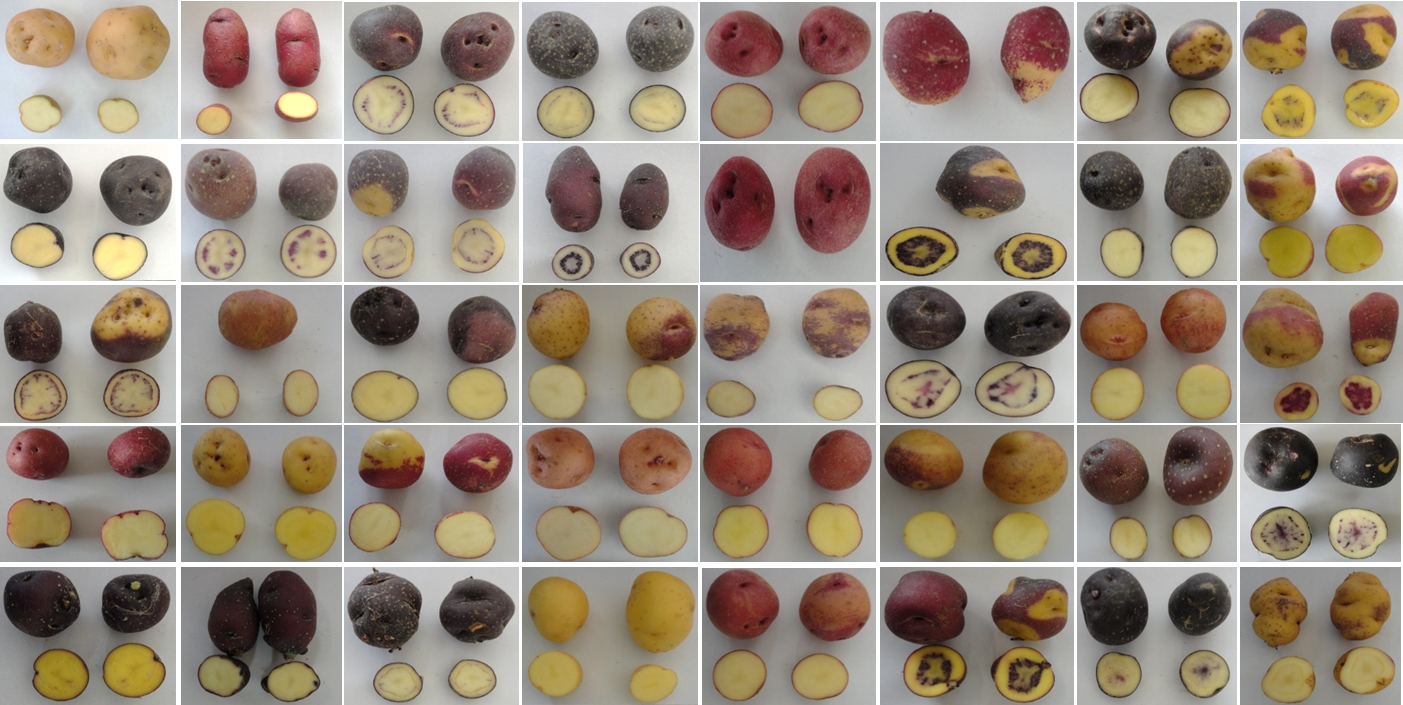
\includegraphics[width=14cm]{Figures/papas_colores.png}

   \caption{Color variation in tuber skin and flesh among CCC accessions.}
    \label{fig:colorpapas}
\end{figure}


\section{Materials and Methods}
The Colombian Central Collection of potatoes (CCC) is one of the most diverse collections in Colombia and the most important source of genetic variability for the improvement of this crop in Colombia \citep{manrique2023defining}. Currently, the CCC clonal collection conserved in the field preserves 1225 accessions, with 68.8\% consisting of  \textit{Solanum tuberosum subsp. andigenum} landraces. Most accessions were collected before 1985. %The passport information is available in GRIN-Global (\url{http://bgvcolombia.agrosavia.co:8026/gringlobal/search.aspx})

\begin{figure}
    \centering
    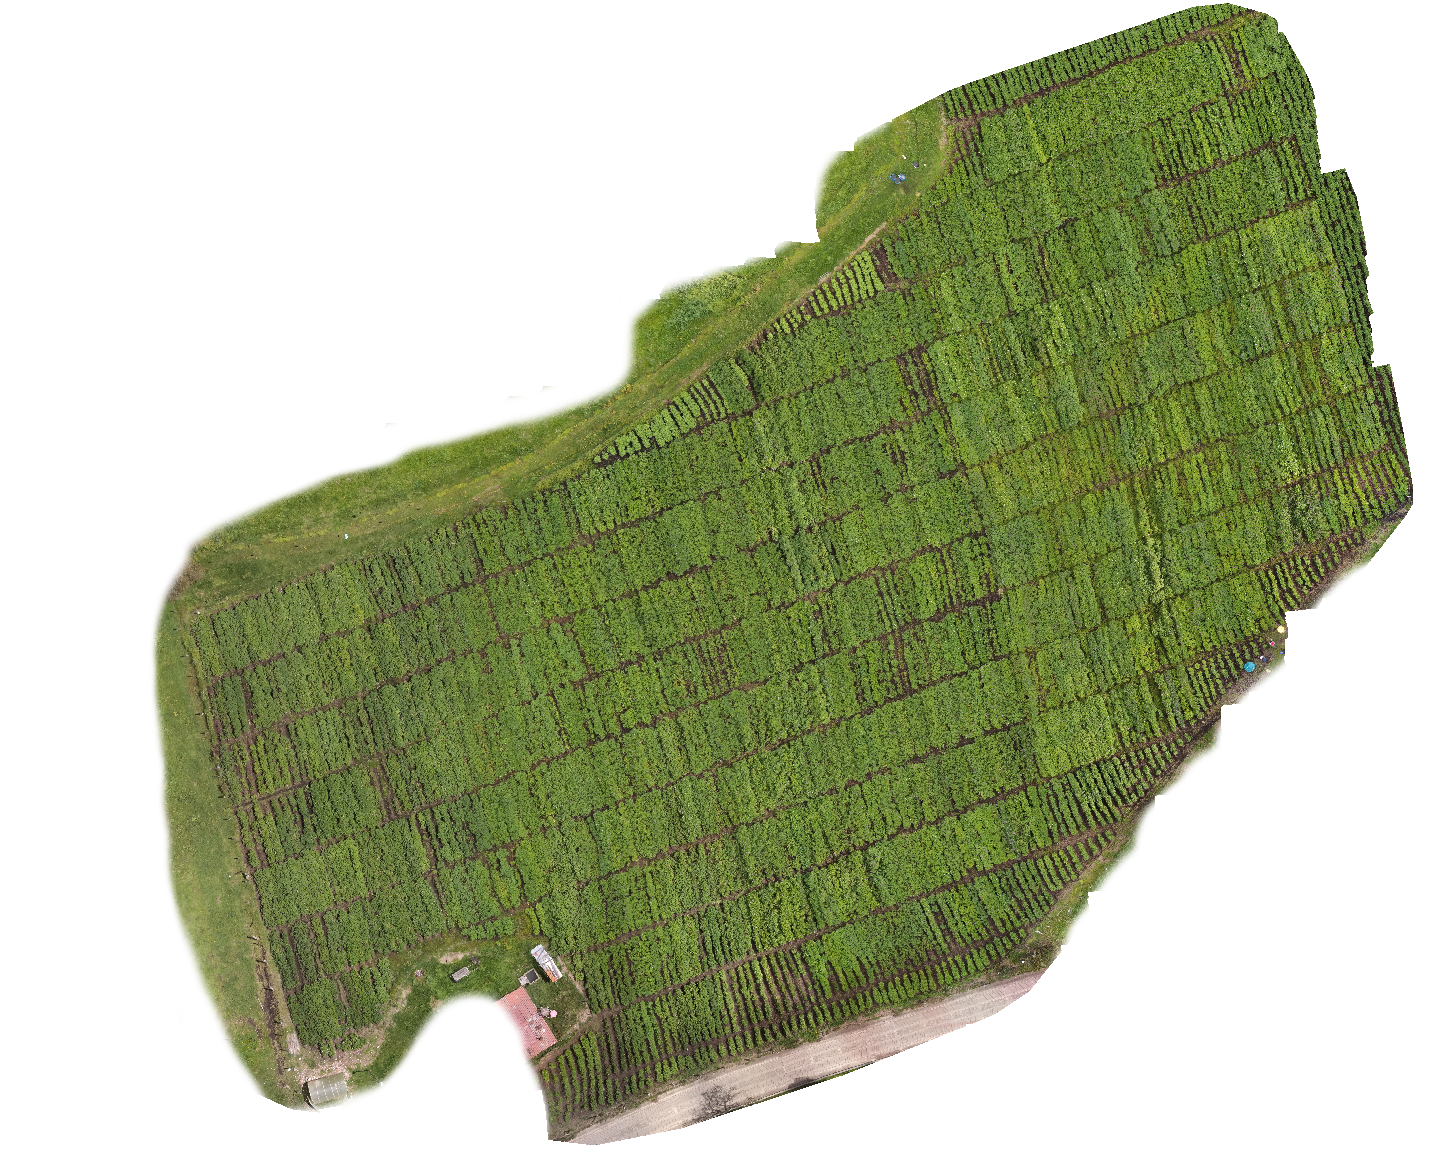
\includegraphics[width=14cm]{Figures/ortofoto092022.png}
    \caption{Aerial image of the CCC field collection in 2022, with each furrow representing an accession, consisting of 20 plants. The orthophoto was created using images captured by a P4 UAV at an altitude of 12 meters in September 2022.}
    \label{cccfield}
\end{figure}

The regeneration of the CCC is conducted annually in the municipality of Zipaquirá (See Figure \ref{cccfield}), located in the department of Cundinamarca, Colombia. This area is situated at an altitude of 2,950 m, with an average temperature of 15°C and a relative humidity of 75\% \citep{Berdugo2017}.

\subsection{Genotypic data}

A set of 657 tetraploid accessions from the CCC, consisting of the  \textit{S. tuberosum} group Andigenum, was previously genotyped \citep{Berdugo2017} using the Illumina Infinium SolCAP SNP array (8303 SNP). The array was processed on the Illumina HiScan SQ system (Illumina, San Diego, CA) at AGROSAVIA, and the ClusterCall R package \citep{Schmitz2017} was used to obtain the dosage genotype calls from the Theta values and(?) raw data values, applying default parameters, and calibration from F1 populations supported by the software. This resulted in a genotype call matrix (0: AAAA, 1: AAAB, 2: AABB, 3: ABBB, and 4: BBBB) for each SNP across all accessions.

%---------------Modificado por Luis Garreta

To ensure data quality and reliability for subsequent GWAS analyses, standard filtering criteria were applied. SNPs with a minor allele frequency (MAF) below 1\% were excluded to eliminate rare variants that may lead to spurious associations due to insufficient statistical power \citep{Anderson2010}. Individuals with a genotype call missing rate (MIND) greater than 10\% were removed to avoid bias introduced by low-quality samples. SNPs with a missing rate (GENO) of $\geq 10\%$ were filtered to maintain marker integrity and reduce imputation noise. Additionally, SNPs with Hardy-Weinberg equilibrium (HWE) p-values below 1e-10 were excluded because extreme deviations may indicate genotyping errors, population structure artifacts, or selection \citep{Wigginton2005}.  These thresholds are commonly used in polyploid GWAS studies and are consistent with established quality control practices \citep{Lu2013,Pavan2020}. Following this filtering process, 4,641 SNPs were retained for downstream genomic analyses.
%PAULA XXX makers


\subsection{Phenotypic data }

Annual regeneration of CCC was used to characterize morphological traits. The field consists of seven square meters allocated for planting 20 seed tubers per accession. Due to the large size of the \textit{S. tuberosum Andigenum} group collection and limited human resources, 600 accessions were evaluated over three years from 2015 to 2017. Color traits were characterized for stem (7 codes), berry (7 codes), and primary and secondary colors of the flower (8 and 9 codes, respectively), tuber skin (9 and 10 codes, respectively), tuber flesh (8 and 9 codes, respectively), and sprout (5 and 6 codes, respectively), using the descriptors proposed by \cite{gomez2000guia}. 

%Carne - flesh, no pulp esto tiene otro significado
%Brote - sprout (no bud)
Additionally, in 2019, color characterization was performed using the fifth edition of the Royal Horticultural Society (RHS) color chart \citep{voss2002royal} to provide a more detailed color evaluation. This change expanded the codes from a maximum of ten options to a set of 884 codes. The chart was used to characterize the following nine traits: stem color (StemC), berry color (BerryC), primary flower color (PCFlower), primary tuber skin color (PCTuberskin), secondary tuber skin color (SCTuberskin), primary tuber flesh color (PCTuberflesh), secondary tuber flesh color (SCTuberflesh), primary sprout color (PCSprout), and secondary sprout color (SCSprout). 


%secondary flower color (SCFlower),
% 10 traits o 9 % Secondary color of the flower no esta???



%\paragraph{HCL space }

Moreover, the color characterization using the RHS color chart was converted to the Hue, Chroma, and Lightness (HCL or LCH) color space, as this model is closely aligned with human color perception and has been used in previous studies on potato color \citep{caraza2020image}.  The values of these LCH traits were derived from the transformation of the values of the potato color traits, measured using the Royal Horticultural Society (RHS) fifth edition color chart (http://rhscf.orgfree.com/) \citep{voss2002royal}, into the three components: L, C, and H, of the Commission Internationale de l'Éclairage (CIE) LCH or CIE{*}L{*}C{*}h color space. Consequently, three components were obtained for each potato color trait, which will be referred to as LCH traits. Thus, the nine potato color traits were transformed into 27 LCH traits, which were used for genomic analyses (Fig. S1). As no outliers were detected, all available data were included in the analysis. 


\subsubsection*{Correlation between two color descriptors}
Two descriptors with different numbers of codes were used to characterize the color traits in CCC in different years. The correlation between the evaluations of both descriptors was calculated for each of the nine color traits using Cramer's V statistic \citep{Lyman1986}. Cramer's V measures the strength of the association between two qualitative variables, with values ranging from 0 to 1. Values below 0.6 indicate a weak association, while values of 0.6 or higher indicate a medium to strong association. To study the genetics underlying color, we selected traits with a medium-to-strong association, indicating genetic influence.


\subsubsection*{Linking Color to Nutritional and Nutraceutical Variables}

This study also examined the association between color traits and nutritional and nutraceutical values using data from a previous study \cite{berdugo2023phenotypic}. The nutritional traits of the potatoes were represented by the Ascorbic Acid Content (AAC), while the nutraceutical traits were: Total Phenol Content (TPC) and Antioxidant Activity (measured by 2.2-Diphenyl-1-picrylhydrazyl Radical Scavenging Activity - DPPH and Ferric Reducing Antioxidant Power - FRAP assays). Given that the nutritional and nutraceutical variables were continuous, and the color traits were categorical, the determination coefficient was applied as a measure of association \cite{nagelkerke1991note}. To evaluate these associations, data from 282 Andigenum accessions in the CCC collection, which included information on both sets of traits, were analyzed.


\subsection{GWAS analysis \label{subsec:GWAS-process} }

% especificar metodologia de GWAS
%1-Control de Calidad de datos
%2-Parametros, Herramientas citar
%3-Estructura como se definio



A previous GWAS study by \cite{Berdugo2017} employed the same genetic dataset and color descriptors as those defined by \cite{gomez2000guia}. In contrast, the present study used the RHS color chart as a phenotype for color characterization, increasing the number of trait values from 30 to 884, thus achieving greater resolution.

We utilized MultiGWAS \citep{Garreta2021}, a tool that integrates the outputs from multiple GWAS methods. Specifically, we incorporated the results from GWASpoly \citep{Rosyara2016} for tetraploid genotypes and GAPIT \citep{Tan2016} for diploid genotypes. The analysis was conducted using the MultiGWAS Full Model (Q+K), which controls for population structure (Q, typically derived from principal component analysis) and kinship (K, based on a genetic relatedness matrix), thereby reducing the likelihood of false-positive associations.

In MultiGWAS, each tool implements a mixed linear model (MLM) (Phenotype ~ Genotype + Q + K), but with method-specific adjustments. GWASpoly adapts the MLM for polyploid data, incorporating population structure and kinship as fixed and random effects, respectively. GAPIT employs a standard MLM, treating the population structure (Q) as a fixed effect (e.g., from PCA) and kinship (K) as a random effect via its kinship matrix. By unifying these approaches, MultiGWAS robustly controls for population stratification and relatedness while detecting marker-trait associations across ploidy levels (diploid and tetraploid).




To address the issue of multiple testing, the MultiGWAS tool applies the Bonferroni correction. However, instead of adjusting the \textit{p-values}, MultiGWAS adjusts the threshold to determine a significant \textit{p-value}. Specifically, this threshold is set to $\alpha/m$, where $\alpha$ represents the significance level and \emph{m} is the number of tested markers from the genotype matrix. The CMPlot library \citep{CMPlot} was used to generate Manhattan and Circos plots to visualize significant SNP markers.


%PAULA - revisa si esto del GSCORE se presenta en los resultados
\subsubsection*{Candidate Marker Identification \label{score}}


Given the evaluation of multiple traits and the integration of results from the four GWAS tools in MultiGWAS, we developed a proprietary scoring function called GSCORE. This function was designed to rank markers by incorporating the outputs from the MultiGWAS. Specifically, GSCORE selected the top 50 markers with the lowest p-values from each tool, resulting in 100 markers (2 tools × 50 markers). GSCORE is calculated as the sum of three weighted terms: inflation factor (I), contributing 70\% of the score. Replicability (R) accounts for 10\%, and significance (S) accounts for the remaining 20\%. The scoring function is represented by the following equation:

\begin{center}
$GSCORE(M)=0.7*I+0.1*R+0.2*S$
\par\end{center}

 $I$ is the inflation factor score, defined as $I=1-|1-\lambda(M)|$, where $\lambda(M)$ is the inflation factor for marker M. This score is the highest when $\lambda(M)$ is close to 1. In addition, $R$ is the number of SNPs shared among the three GWAS tools. Finally, $S$ is a binary value (1 or 0) that indicates whether the SNP is significant (p-value < threshold). Marker $M$ achieves a high $GSCORE$ when it has an inflation factor $\lambda(M)$ close to one, identifies a large number of shared SNPs across tools, and is statistically significant. In contrast, the score is low if $\lambda(M)$ is either too low (close to 0) or excessively high, identifies few shared SNPs, or is not significant. In other scenarios, the score is determined by a balance between the inflation factor, shared SNP count, and significance. This approach prioritizes markers that are statistically robust, consistent across tools, and highly significant.


\subsubsection*{Marker annotation\label{subsec:OwnScoreFunction}}
Markers were annotated by taking information from the Potato Genome Sequencing Consortium (PGSC) public data based on the double monoploid \textit{S. tuberosum} Group Phureja from assembly DMv6.1\citep{Pham2020} obtained from the SpudDB website. Annotation was performed by associating marker identifiers with information from both the high confidence gene models annotation, the InterProScan assigned GO terms for the working gene models, the InterProScan search results for the working gene models, and the SolCAP 69 K SNP positions on the DMv6.1 assembly available in SpudDB. Furthermore, for each trait, the amino acid sequences were analyzed using BlastKOALA \citep{kanehisa2016blastkoala} for KEGG mapping to identify common functional categories among the significant markers.



\subsection{Heritability}

Narrow-sense heritability \emph{$h{{}^2}$,} defined as the proportion of phenotypic variance explained by additive effects \citep{Campos2015}, was estimated for all LCH components using by the following equation:
\begin{center}
$h{{}^2}=\dfrac{\sigma_{a}^{2}}{\sigma_{y}^{2}}$
\par\end{center}

where $\sigma_{a}^{2}$ denotes additive genetic variance and $\sigma_{y}^{2}$ denotes phenotypic variance. These variances were obtained by fitting a whole-genome regression model using Bayesian regression implemented in the BGLR package in R \citep{Campos2014}. %(\url{https://github.com/gdlc/BGLR-R/blob/master/inst/md/heritability.md}).


\subsection{Genomic Prediction (GP)}
We used 12 Genomic Prediction (GP) models with a large number of genetic markers to generate genomic estimated breeding values (GEBVs) for each of the 27 LCH traits. 
The genomic prediction (GP) models encompassed three categories: parametric models—including Genomic Best Linear Unbiased Prediction (GBLUP), Estimated Best Linear Unbiased Prediction (EGBLUP), Ridge Regression (RR), and Least Absolute Shrinkage and Selection Operator (LASSO); semiparametric models—comprising Reproducing Kernel Hilbert Spaces (RKHS), Random Forest (RF), and Support Vector Machine (SVM); and Bayesian models—including Bayesian Ridge Regression (BRR), Bayesian LASSO (BL), Bayes A, Bayes B, and Bayes C.
%The GP models included parametric (Genomic Best Linear Unbiased Prediction GBLUP, Estimated Best Linear Unbiased Prediction EGBLUP, Ridge Regression RR, and Least Absolute Shrinkage and Selection Operator LASSO), semiparametric ( Reproducing Kernel Hilbert Spaces  RKHS, Random Forest RF, and Support Vector Machine SVM), and Bayesian (Bayesian Ridge Regression BRR, Bayesian LASSO BL, Bayes A, Bayes B, and Bayes C) models. 
Additionally, to identify the optimal number and type of markers for estimating GEBVs, various subsets of markers generated through GWAS were tested.
The R package for the Breed Wheat Genomic Selection Pipeline (BWGS) \citep{Charmet2020} was used. Furthermore, 5-fold cross-validation, repeated five times, was employed to assess the performance of the 12 models for each LCH trait. The parameter values for running each model were set to the default settings provided by the BWGS library.

\subsubsection{GP using marker subsets}


To determine the optimal number of markers for genomic prediction (GP) of each LCH color trait component, GP was conducted using subsets containing varying numbers of markers. These markers were selected based on GWAS results and prioritized according to their relevance using our custom GSCORE scoring function (see Section \ref{score}). 








\section{Results}

%\subsection{Relationships between potato color traits measured with two color descriptors}
%PAULA: por revisar

The distribution for the three components of the color traits can be seen in Figure S1 in the supplementary information.


\subsection{Correlation between descriptors}

The correlations between the values of the color traits measured with the two color descriptors over different years are presented in Figure \ref{fig:Correlations-years} A. Among the traits, only berry color and primary tuber flesh color exhibited weak correlations, leading to their exclusion from the genetic study. In contrast, the remaining seven color traits showed moderate to strong correlations, ranging from 0.65 to 0.97. Although some color traits were correlated with others, all moderate to strong correlations, as expected, were concentrated along the diagonal of the correlation matrix. In particular, there were correlations between primary and secondary tuber skin colors, between primary tuber skin color and both primary and secondary tuber flesh colors, and between primary and secondary sprout colors.




%shows the correlations between the values of the color traits measured in the first and second year, where high correlations ($>$70\%) are observed for the traits CPBrote, CPFlor, CPTuber, and CSBrote; good correlations ($>$50\%) for CPulpa, CSCarne, CSTuber, and CTallo; and a low correlation for the trait CBaya.


\begin{figure}[h]
    \centering
    
    %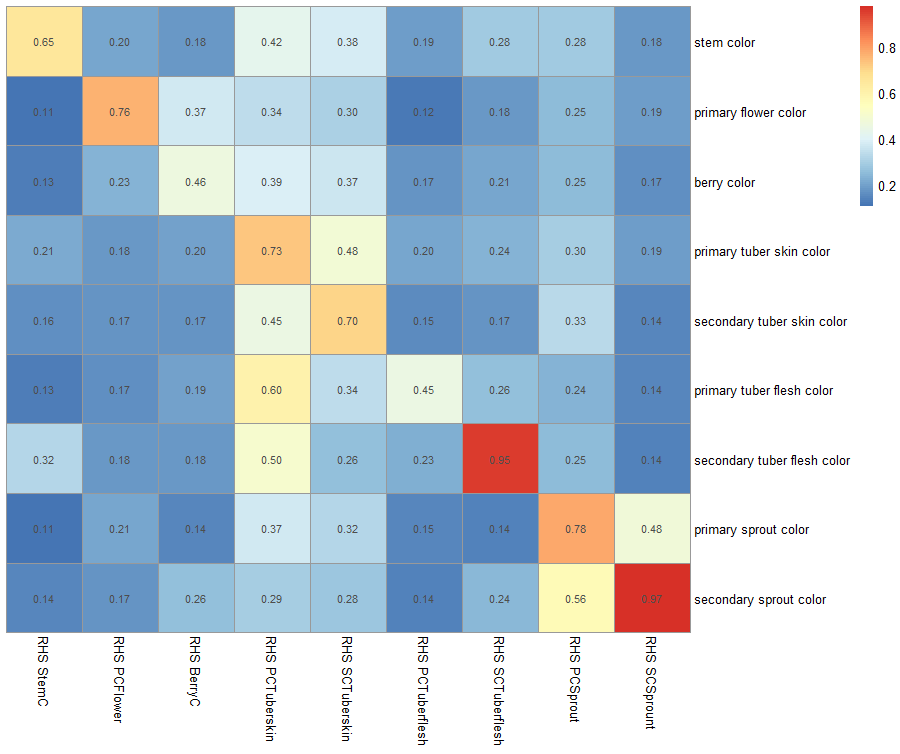
\includegraphics[width=12cm]{Figures/Correlacion_Traits.v2.png}
    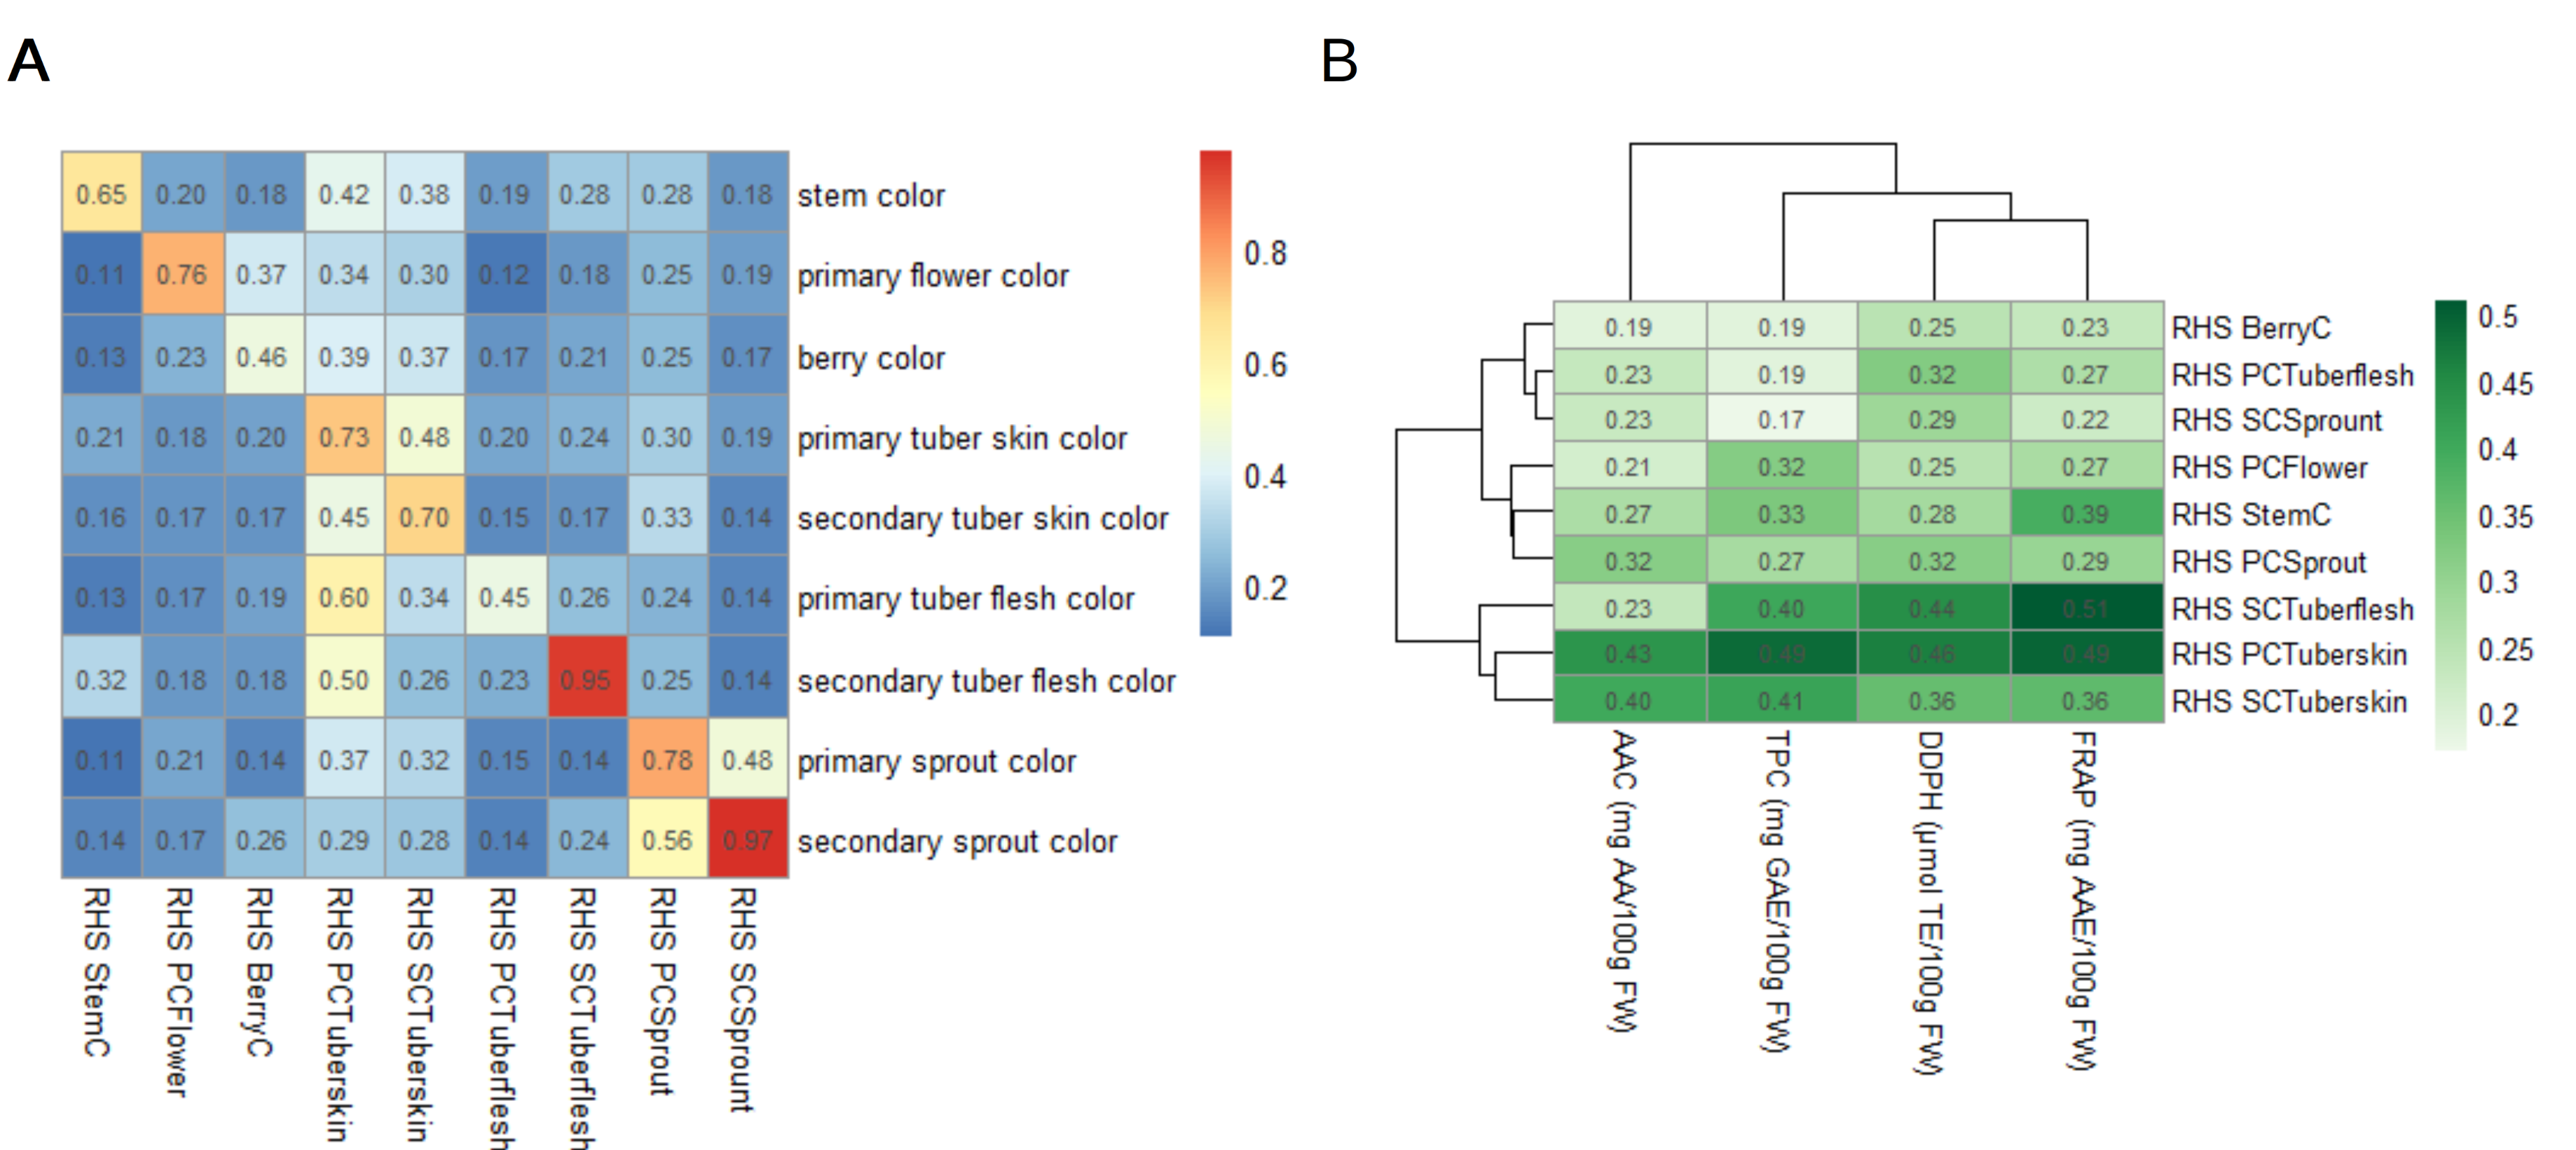
\includegraphics[width=12cm]{Figures/FigPanel_correlacion.png}
\caption{\textbf{A.} Heatmap showing the correlation matrix of potato color traits in CCC accessions, derived form  descriptors by \cite{gomez2000guia} and measured with RHS \citep{voss2002royal} color chart. The color bar is located in the top right, with blue indicating low correlation values and red representing high correlation values. \textbf{B.} Heatmap showing the determination coefficient between nutritional (AAC) and nutraceutical (TPC, DPPH, and FRAP assay reported by \citep{berdugo2023phenotypic} components and potato RHS color traits.  The color bar is located at the top right, with the intensity of green representing the determination coefficient. \label{fig:Determination coefficient} \label{fig:Correlations-years}}. 

\end{figure}


\subsubsection{Linking Color to Nutritional and Nutraceutical Variables}
In Figure \ref{fig:Determination coefficient} B, the heatmap presents the determination coefficient $R^2$ between the color traits measured using the RHS color scale and nutritional/nutraceutical variables. $R^2$ below 0.3 reflect a weak association (blue cells), while $R^2$ between 0.3 and 0.51 reflects a moderate association between color traits and nutritional variables (yellow and red). Three specific traits—the secondary color of the tuber flesh and the primary and secondary colors of the tuber skin—exhibited notable associations with nutritional variables. Antioxidant activity (measured using FRAP and DPPH assays) showed the strongest correlation with these traits. Additionally, Total Phenol Content and Ascorbic Acid Content demonstrated the highest association with the primary color of the tuber skin. Stem color, meanwhile, showed a moderate association with antioxidant activity and Total Phenol Content.








\subsection{GWAS  Analysis}

%\subsubsection{SNPs associated with LCH traits}

 GWAS analysis identified 21 significant SNPs associated with five traits: ten related to the secondary color of the tuber flesh, four to the primary color of the flower,  three to the primary color of the sprout, two to the secondary color of the sprout, and two to the stem color. Manhattan plots for all seven traits are presented in Figure \ref{fig:GWAS-Top-Markers-GSCORE} (A-G). The most significant SNPs were associated with the Hue component and secondary color of the tuber flesh trait. %However, for the secondary color of the sprout, significant SNPs were also identified for the Chroma and Lightness components.


Notably, chromosome 2 accounted for 28.5\% of the significant SNPs, followed by chromosomes 1 and 11, each contributing 19\% and 14.29\%, respectively. 
A Circos plot (Figure S2) combines the data for all seven traits and presents the density of SNP markers for chromosomes, allowing the visualization of SNP co-occurrence across different traits. 




\begin{figure}[H]
\begin{centering}
\begin{center}
%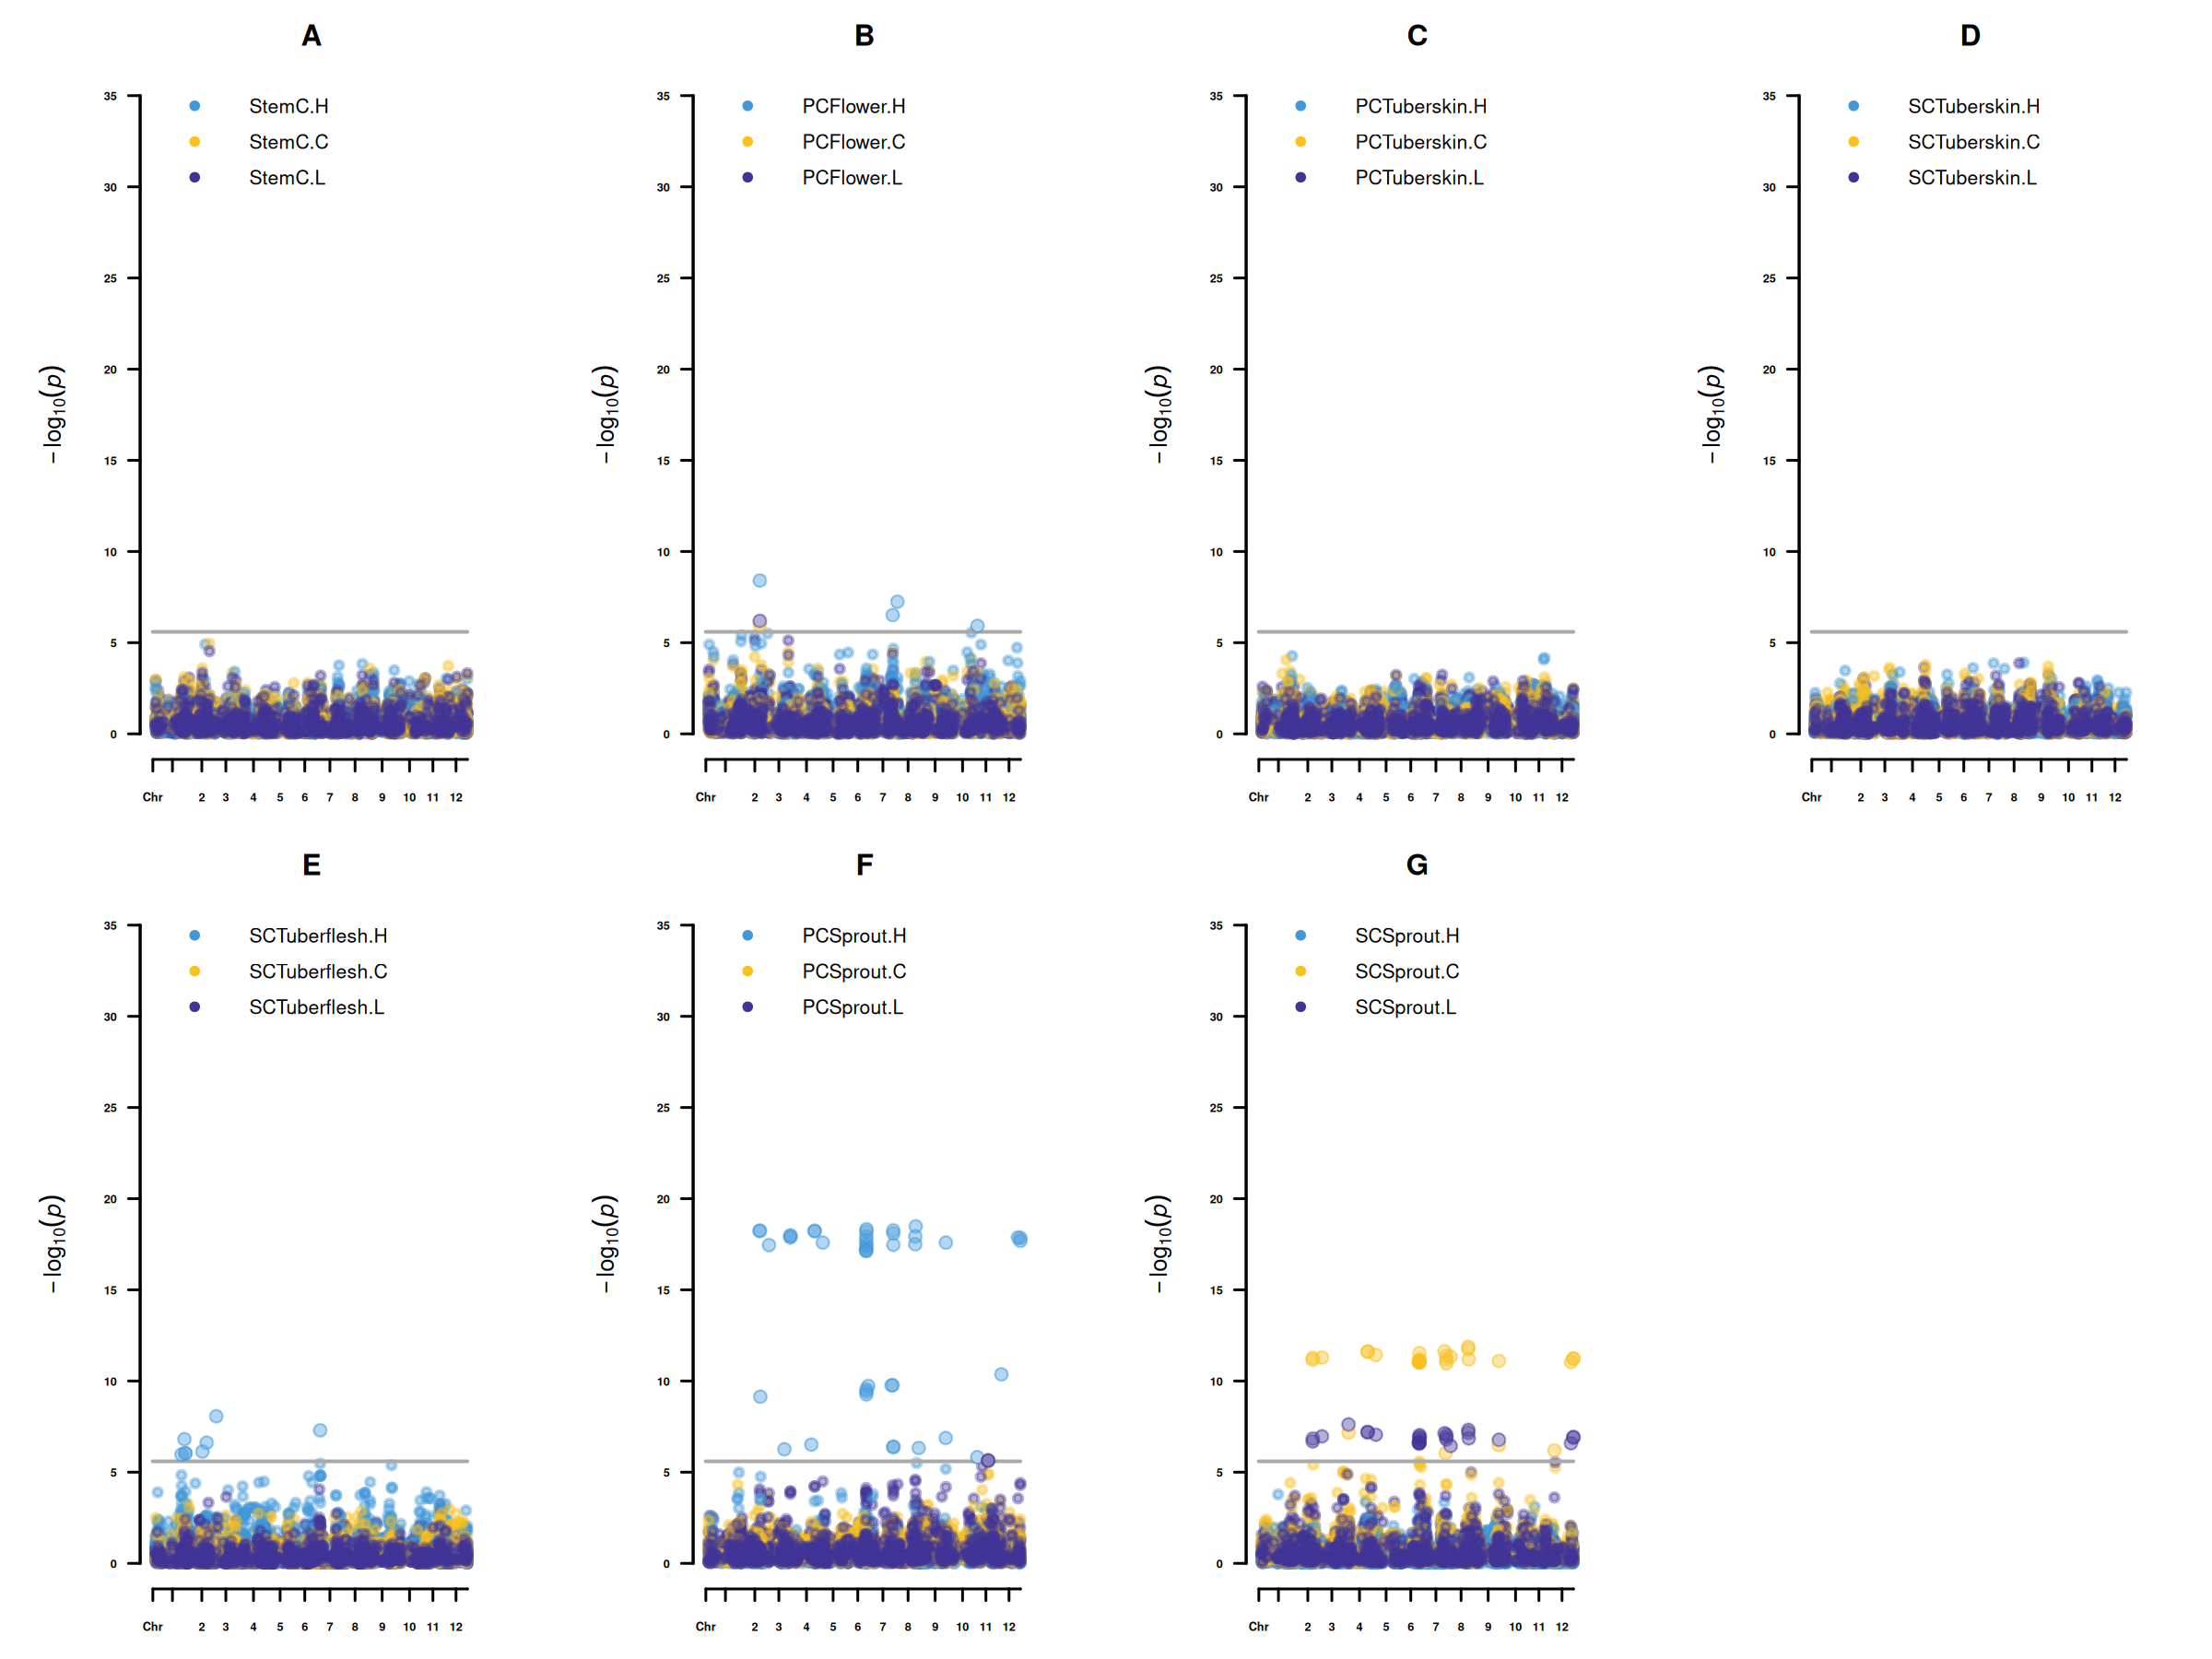
\includegraphics[width=14cm]{Figures/Manhattan.png}
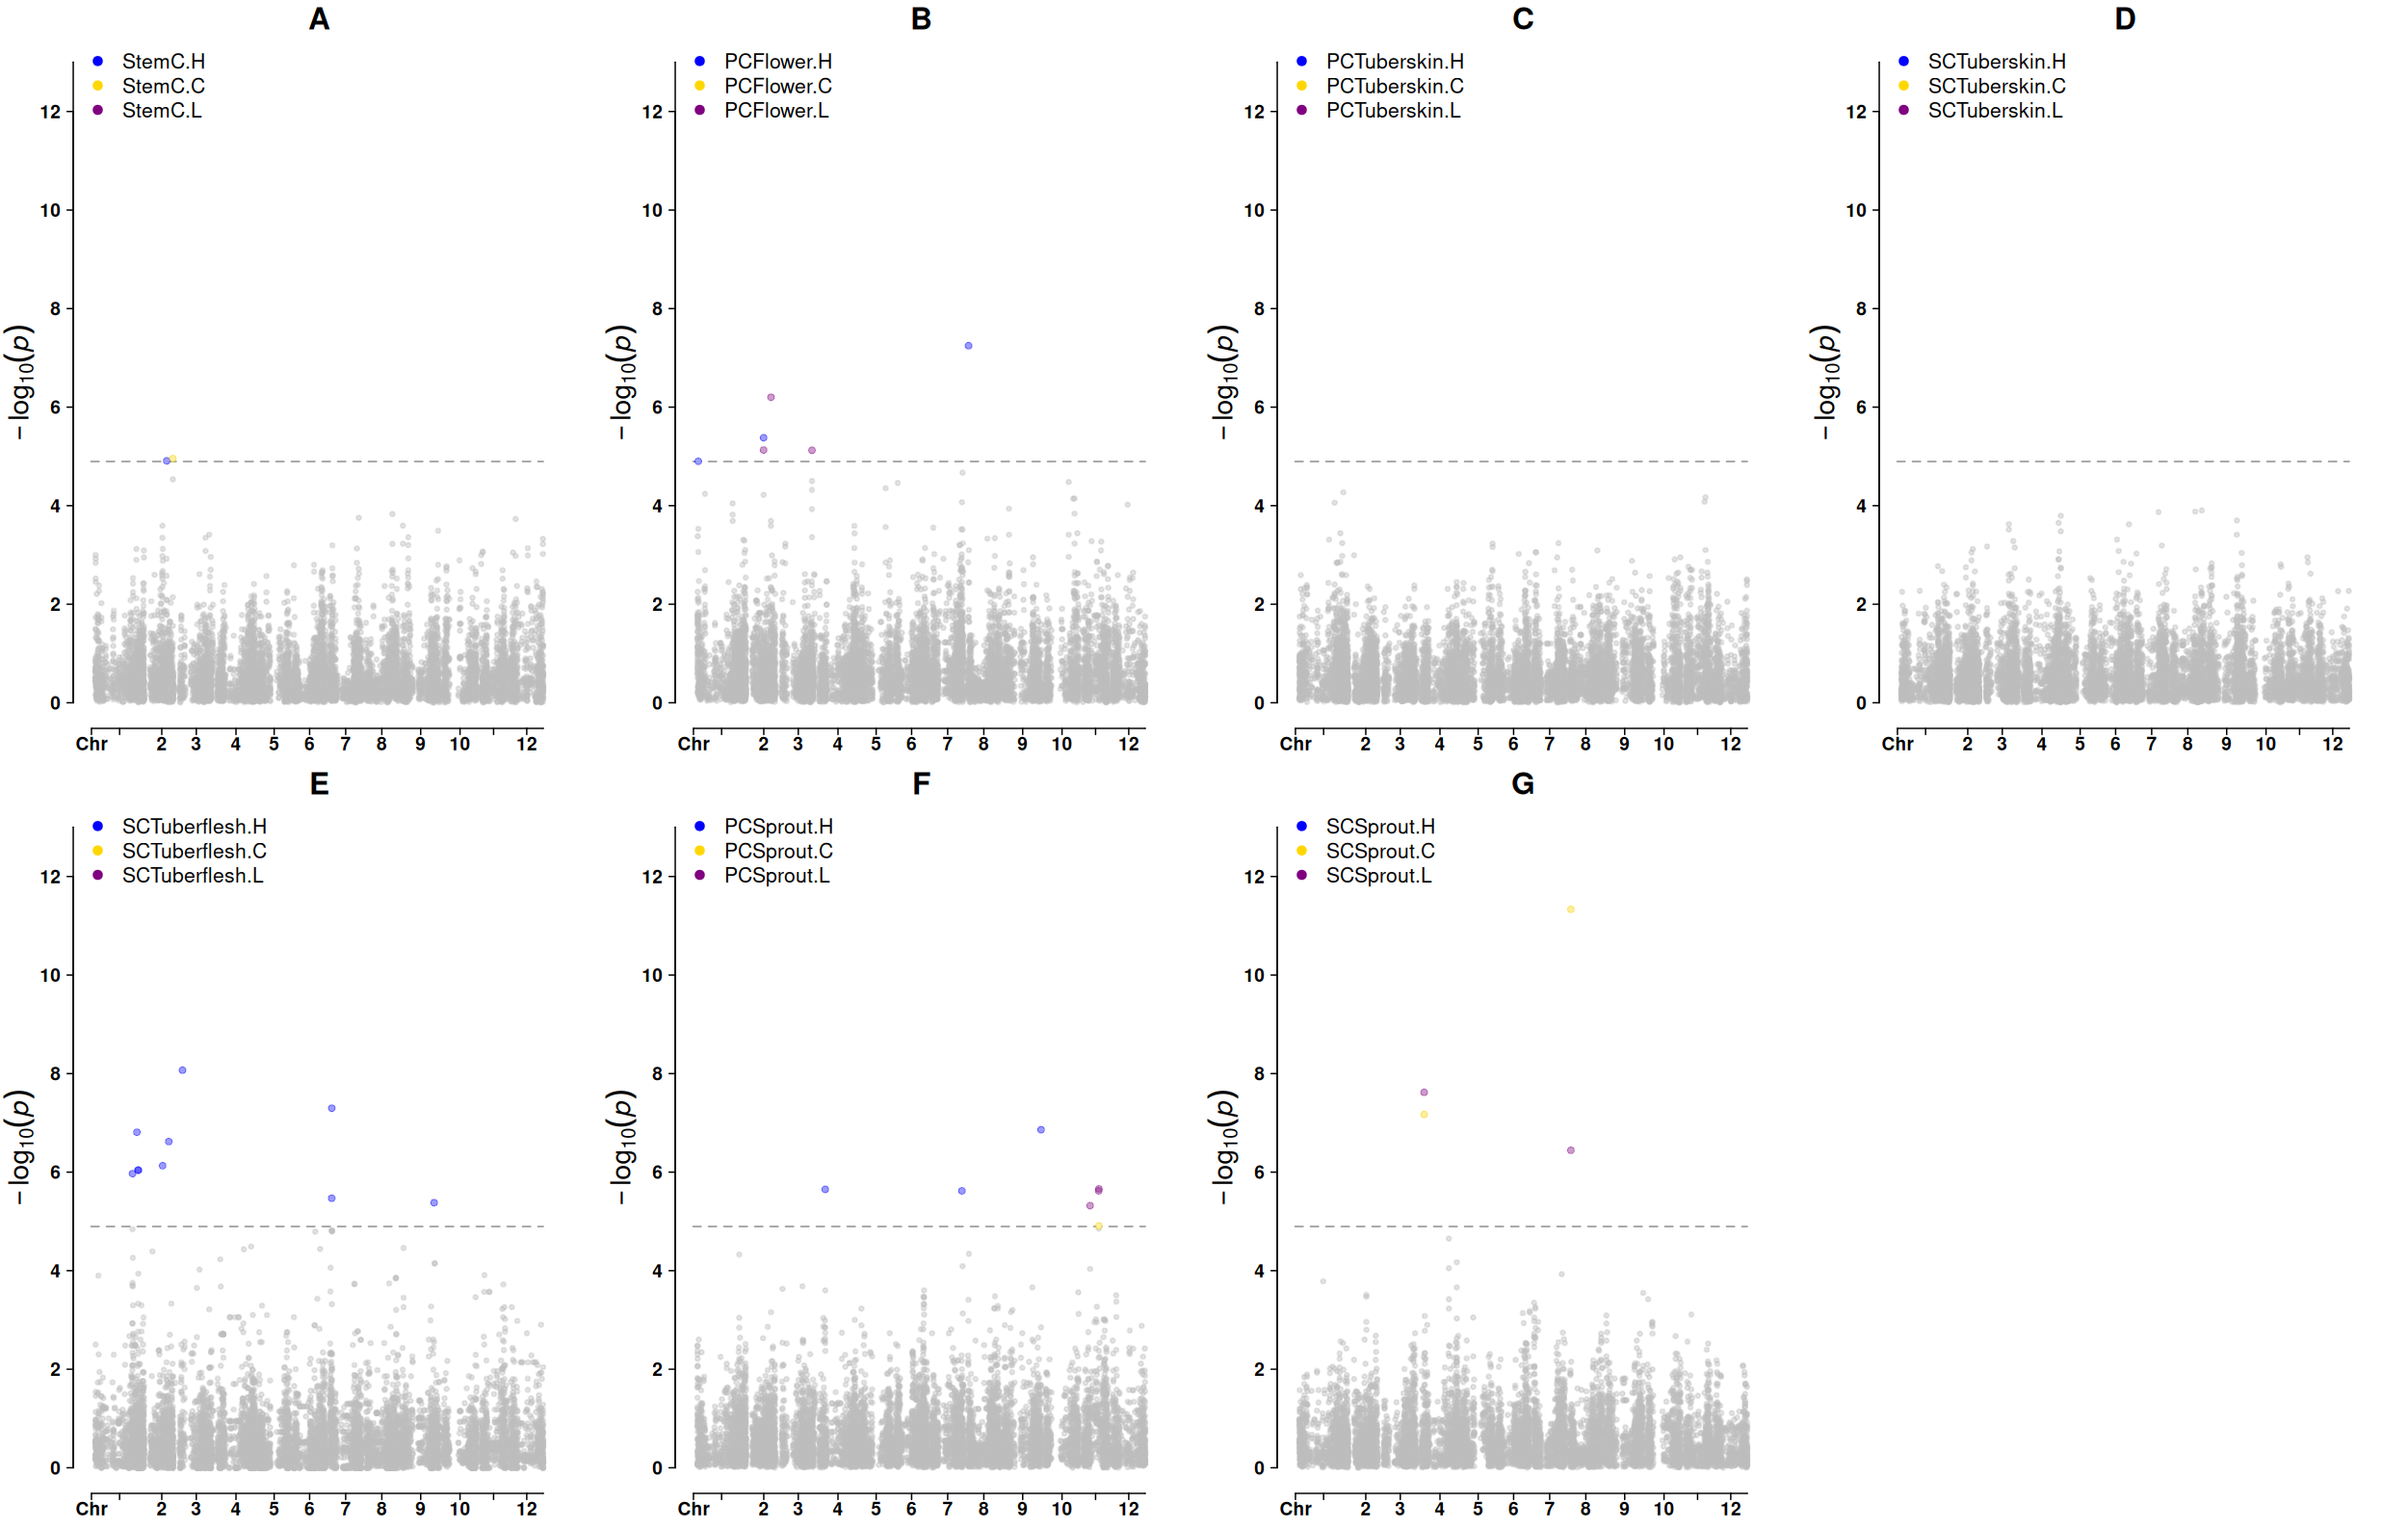
\includegraphics[width=15cm]{Figures/Fig4v4.png}

\par\end{center}%

\par\end{centering}
\caption{(A-G) Manhattan plots show the markers linked to LCH traits, with colors indicating the significant SNPs associated with each LCH color component.\label{fig:GWAS-Top-Markers-GSCORE}}
\end{figure}



A total of 21 significant associations were detected across the nine HCL components that corresponded to five traits. These associations involved 21 SNP markers annotated with 21 genes, represented by a total of 33 transcripts.  A total of eight functional pathway categories were identified based on genes annotated with significant SNPs: seven belonged to the metabolism category and one to the genetic information processing category. Information on the primary annotations linked to these markers, as retrieved from the SPUD database, is provided in Supplementary Table 1, and the specific functional categories per trait are provided in Supplementary Table 2.  

Moreover, GWASpoly and GAPIT identified 50\% of the significant SNPs, with both tools jointly predicting nine SNPs, representing 42.85\% of the total. Although no common SNPs were found across the different traits, four SNPs were associated with distinct HCL components of the same trait.%. 


\subsection{Heritability}

 In general, most traits exhibit high average heritability values ($\geq 0.5$), with the exception of the secondary color of the sprout. Figure \ref{fig:Heritabilities} A. shows the heritability of the selected LCH traits. The primary color of the flower and secondary color of the tuber flesh exhibited high heritability values (greater than 0.9) for the two LCH traits. Furthermore, the color of the stem showed heritability of $\geq 0.8$.

\subsection{Genomic Prediction}

The results for genomic prediction (GP) using all 4,641 markers from the potato dataset are in Figure \ref{fig:Heritabilities} B. Predictive ability corresponds to the correlation between the observed phenotype values and the predicted genomic estimated breeding values (GEBV) in the validation set. Primary flower color and stem color exhibited the highest predictive abilities, followed by the primary color of the tuber skin and the primary color of the tuber sprout. However, the secondary colors of sprouts, tuber flesh, and tuber skin showed low predictive ability.

\begin{figure}[H]
\begin{centering}
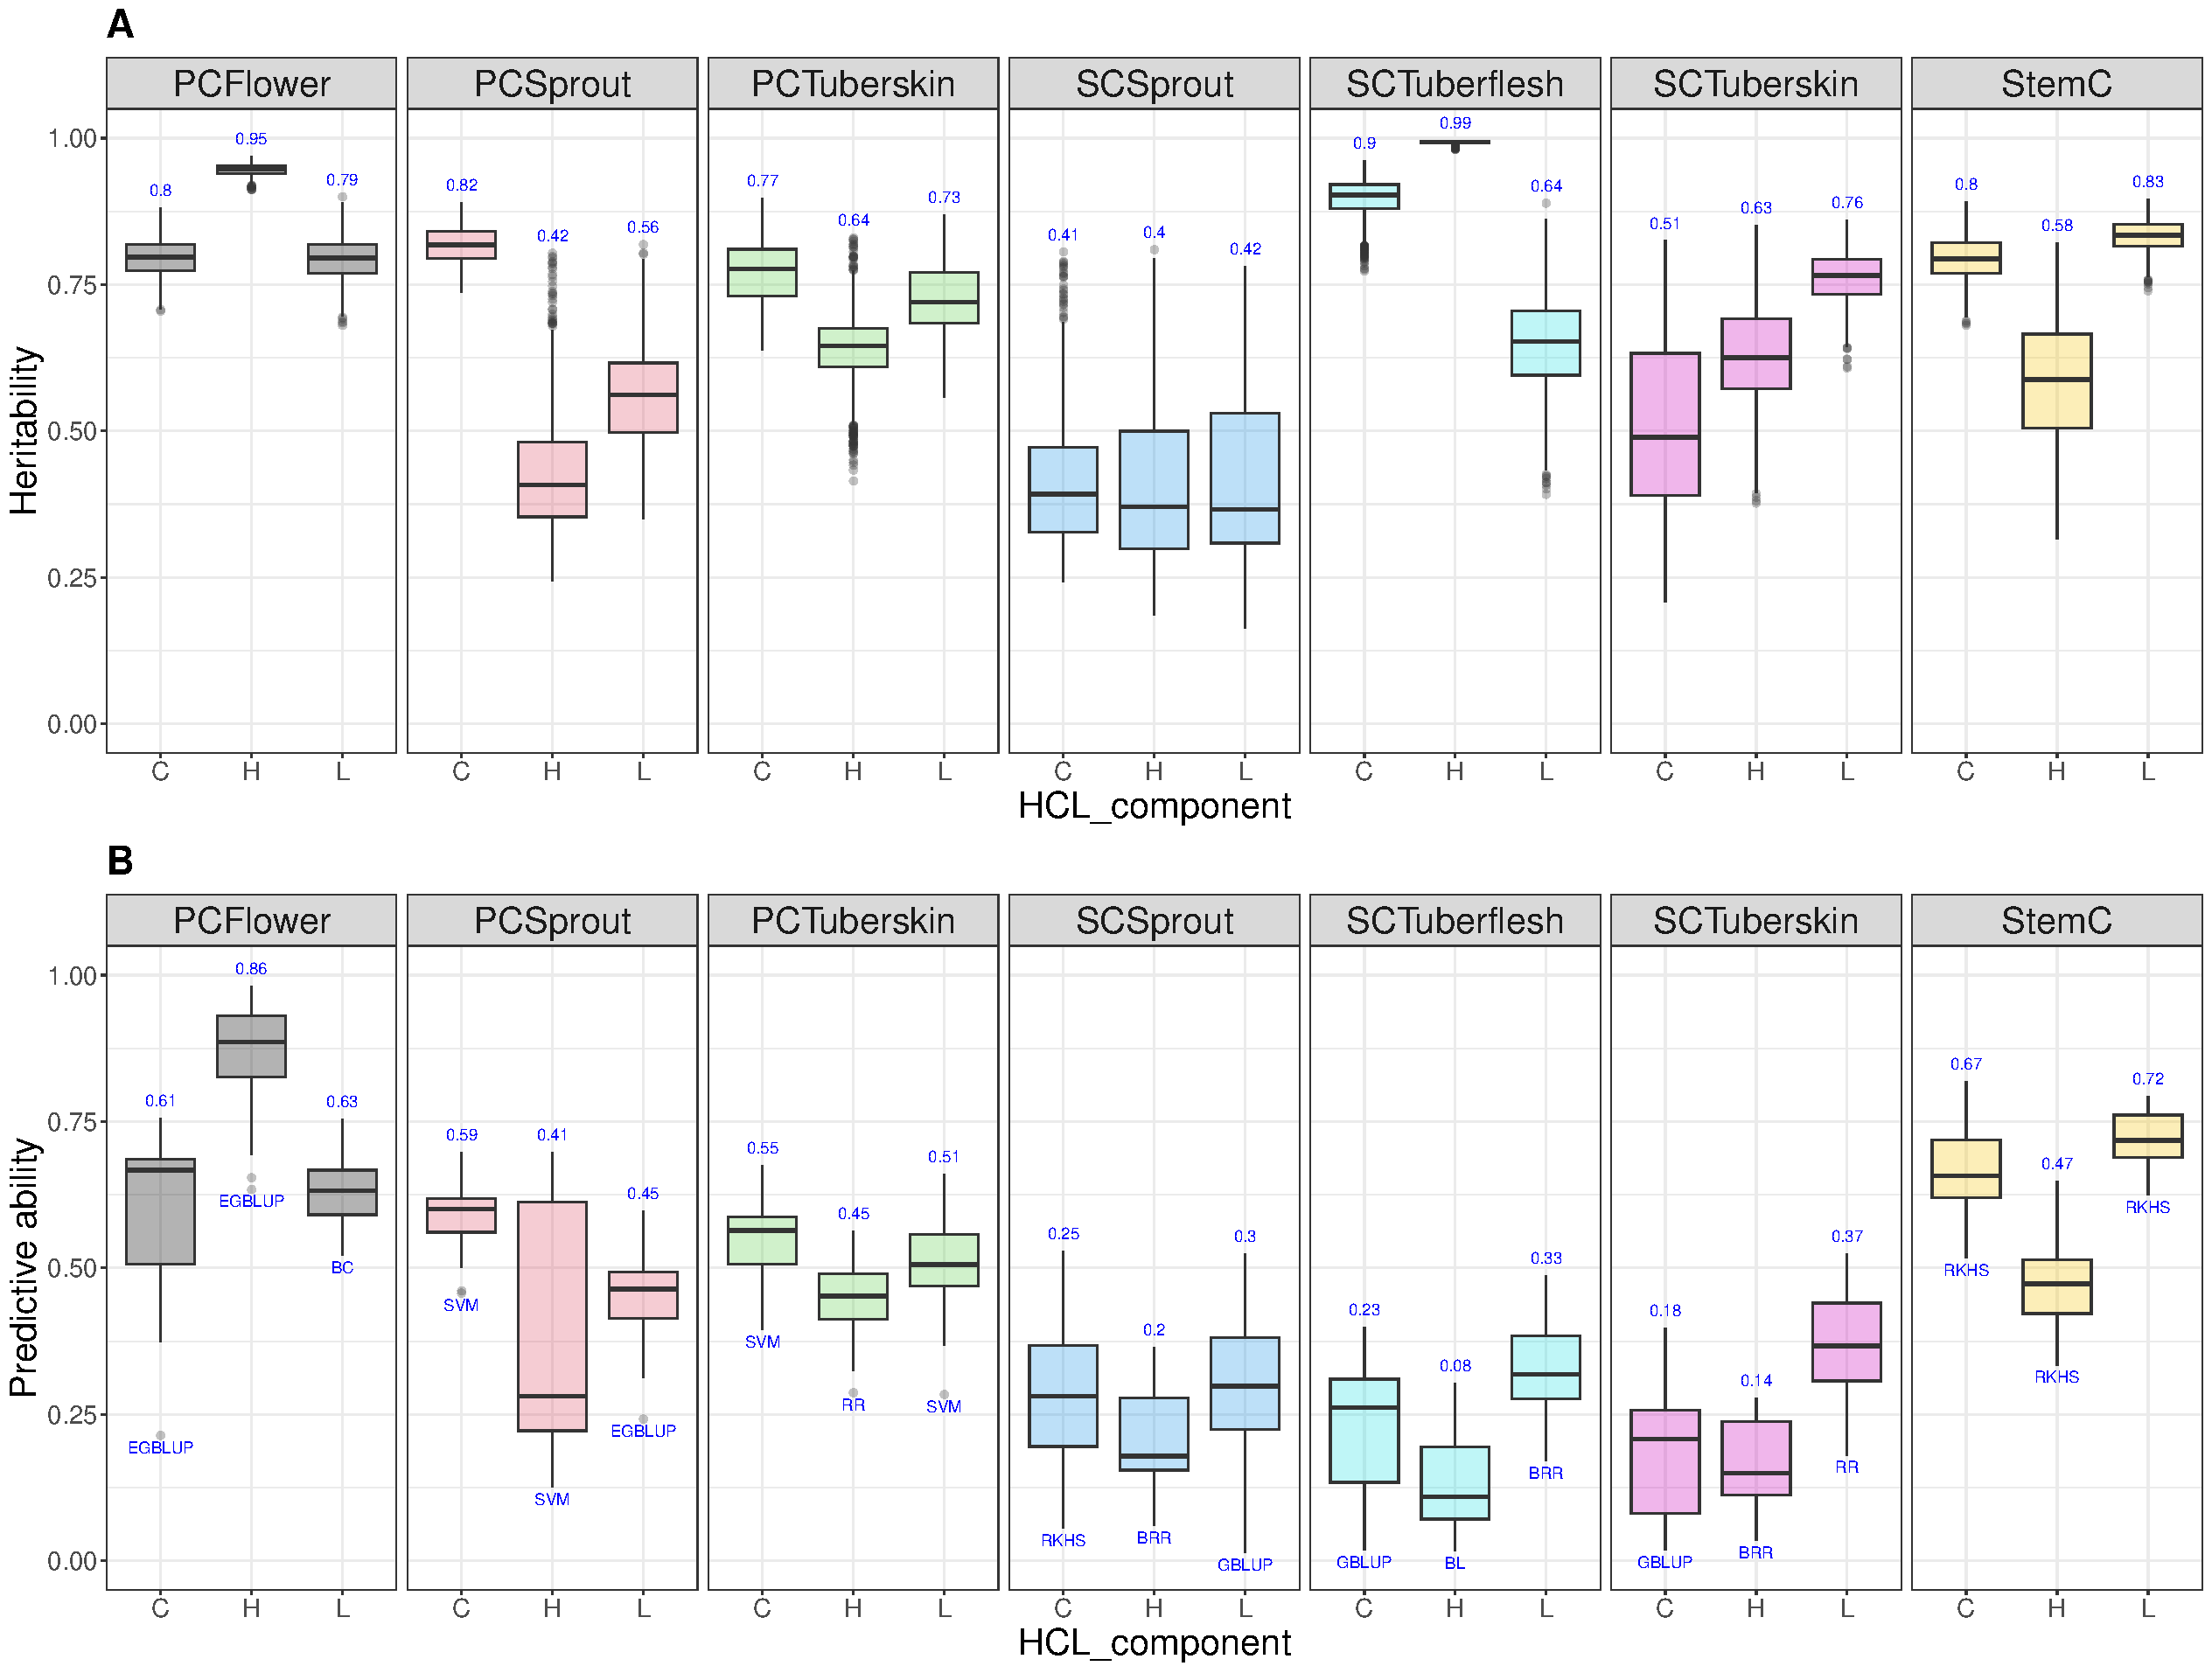
\includegraphics[width=15cm]{Figures/ColorPapa_H_PA_boxplots.v2.pdf}
\par\end{centering}
\caption{\textbf{A . Estimated heritabilities for LCH traits.} At the top of each division is the name of the potato color trait, whereas at the bottom is the LCH component of that trait being evaluated. At the top of each boxplot, in blue, is the mean value of heritability \label{fig:Heritabilities}. \textbf{B. Predictive abilities of GS models for LCH traits.} Comparison of genomic predictions for LCH components using the full set of markers.  The horizontal axis represents the three LCH components for each of the seven potato color traits, while the vertical axis displays the predictive ability values ranging from 0 to 1. The mean predictive ability is displayed at the top of each boxplot, while the model that achieved the best prediction is indicated at the bottom.}
\end{figure}

\subsubsection{GP using marker subsets}

Genomic prediction was performed using marker subsets representing 5\%–100\% of the 4,641 SNPs. Predictive ability, assessed by the Pearson correlation between observed phenotypes and genomic estimated breeding values (GEBVs), varied by trait and marker density (see Figure S3).

In general, predictive ability increased rapidly with marker density up to 40\%-50\% of the total set, after which gains plateaued, indicating diminishing returns. This pattern held across most color traits and LCH components (Hue, Chroma, Lightness), suggesting that a moderate number of well-distributed, informative SNPs can achieve predictive performance comparable to that of the full marker set.

Stem color and primary flower color traits consistently showed higher predictive abilities, with correlations nearing 0.75 at full marker density. In contrast, secondary traits, such as secondary tuber flesh or sprout color, showed lower predictive values, even with more markers. This variability reflects differences in genetic architecture, with some traits likely controlled by major loci and others influenced by more polygenic and complex effects.

These results support the feasibility of cost-effective genomic selection for tetraploid \textit{Andigenum} potatoes by using an optimized SNP subset. The top 50\% of markers, selected via the GSCORE metric (Section 2.3), effectively captured the relevant genetic variation, enabling accurate predictions while reducing the computational demand.






%% Figura suplementaria






\section{Acknowledgments and Funding}

%Proyecto postdoctoral Luis - Minciencias


\bibliography{referencias}% common bib file
%% if required, the content of .bbl file can be included here once bbl is generated
%%\input sn-article.bbl


\end{document}
